\chapter{Introduction} \label{chap:intro} 
Modern applications of machine learning in a broad range of industrial and consumer-facing systems have become ubiquitous.
Most interactions with daily technologies now intrinsically involve 
a request to some ``smart`` system in the ``cloud'', 
where those interactions range from
a request for map directions 
to simply loading a webpage.
Neural network models, and the recent advances of deep learning,
have enabled these systems that 
make such applications possible.
These models have achieved
human-level performance on learning tasks
including image classification~\citep{resnet,alexnet}, image segmentation~\citep{segmentation}, video analysis~\citep{zhang2016video}, text understanding and generation~\citep{bert,gpt}, and have slowly begun to solve more fundamental scientific problems such as protein folding~\citep{protein} drug discovery~\citep{drugdisc}, and medical diagnosis~\citep{diag}.
While this performance is largely attributed to model size,
the abundance of high quality training data
has equally contributed to real world performance,
enabling model training over millions of real world samples~\citep{imagenet,laion},
and potentially billions of synthetic samples via environment simulation~\citep{mcts}.

While deployment in some domains (recommender systems, object detection) may benefit almost unconditionally from this vastly expanded capability, rightful hesitancy has limited their widespread use in particular applications where impacts on individuals, people, or environments may be at stake.
These ``last mile'' concerns take a few forms.
% Because a completely accurate model is still out of reach, an important question that needs to be answered is: which inputs or individuals are being given incorrect outcomes, and why?
% maybe a sentence suggesting unlearning/removal
In mission critical applications such as medical diagnosis, 
the impact of an error can be extremely large,
even if a misprediction happens extremely infrequently.
Additionally, large scale model training and architecture search
can require exorbitant amounts of energy producing high emissions,
and their scale can limit participation
to only large actors with vast existing resources~\citep{anthony2020carbontracker}.
The accessibility and effectiveness of these models can also vary significantly based on the training data, and disparate outcomes can be exacerbated by existing social inequity.

While existing human or ``natural'' systems that these models aim to assist are not perfect, 
our real world has developed norms and regulations that 
enable them to function.
A medical diagnosis might require a physician to explain what symptoms led them to that particular conclusion.
Energy metering and carbon taxes may be applied to limit
emissions.
Regulatory satisfaction may require 
analysis proving equal opportunity,
or that specific protected classes
are not used in decision making.
% Specifically, these can include ideas as simple as the Hippocratic Oath and medical malpractice insurance, to asking your doctor what symptoms lead them to a particular diagnosis.
These ideas are difficult to directly translate to automated machine learning systems,
but proxies have been identified that we can build upon.

These norms and regulations answer a number of questions we may also try to pose to our machine learning models.
What is the cost to learn this task?
What led to this particular outcome?
Why is this outcome different from another?
% We will explore how these questions can be formulated concretely. 

If the answer to these questions is negative or unknown,  follow-up questions all take an interesting form:
Can we learn a smaller model with similar performance? 
Can we identify the most important features? 
Which individuals or groups are being treated unfairly, and can we change that?
These questions ask us to identify a \textit{subset} of some relevant set, dependent on setting, and this identification is our focus here.

% Moving specifically to machine learning methods,
Taking a step back, let's take a look at a representative system. Figure~\ref{fig:dl} illustrates a typical learning pipeline. 
A dataset is collected and used to train a model, by minimizing the error over
those samples in the dataset (top).
A ``sample'' can be a single measured value, or it can
be a large, highly structured object with many ``features.''
The model is made up of some ``parameters'' that are 
tuned during training to learn a good predictor over the training dataset.
This model is then used to predict, or \textit{infer}, on new
data seen ``in the wild'' (bottom).
Our questions above are formally asking to identify \textit{subsets of these objects}: is a subset of the model parameters sufficient for learning? Which subset of the features are important for a prediction? Which subset of the dataset exhibit a specific attribute?
\begin{figure}
    \centering
    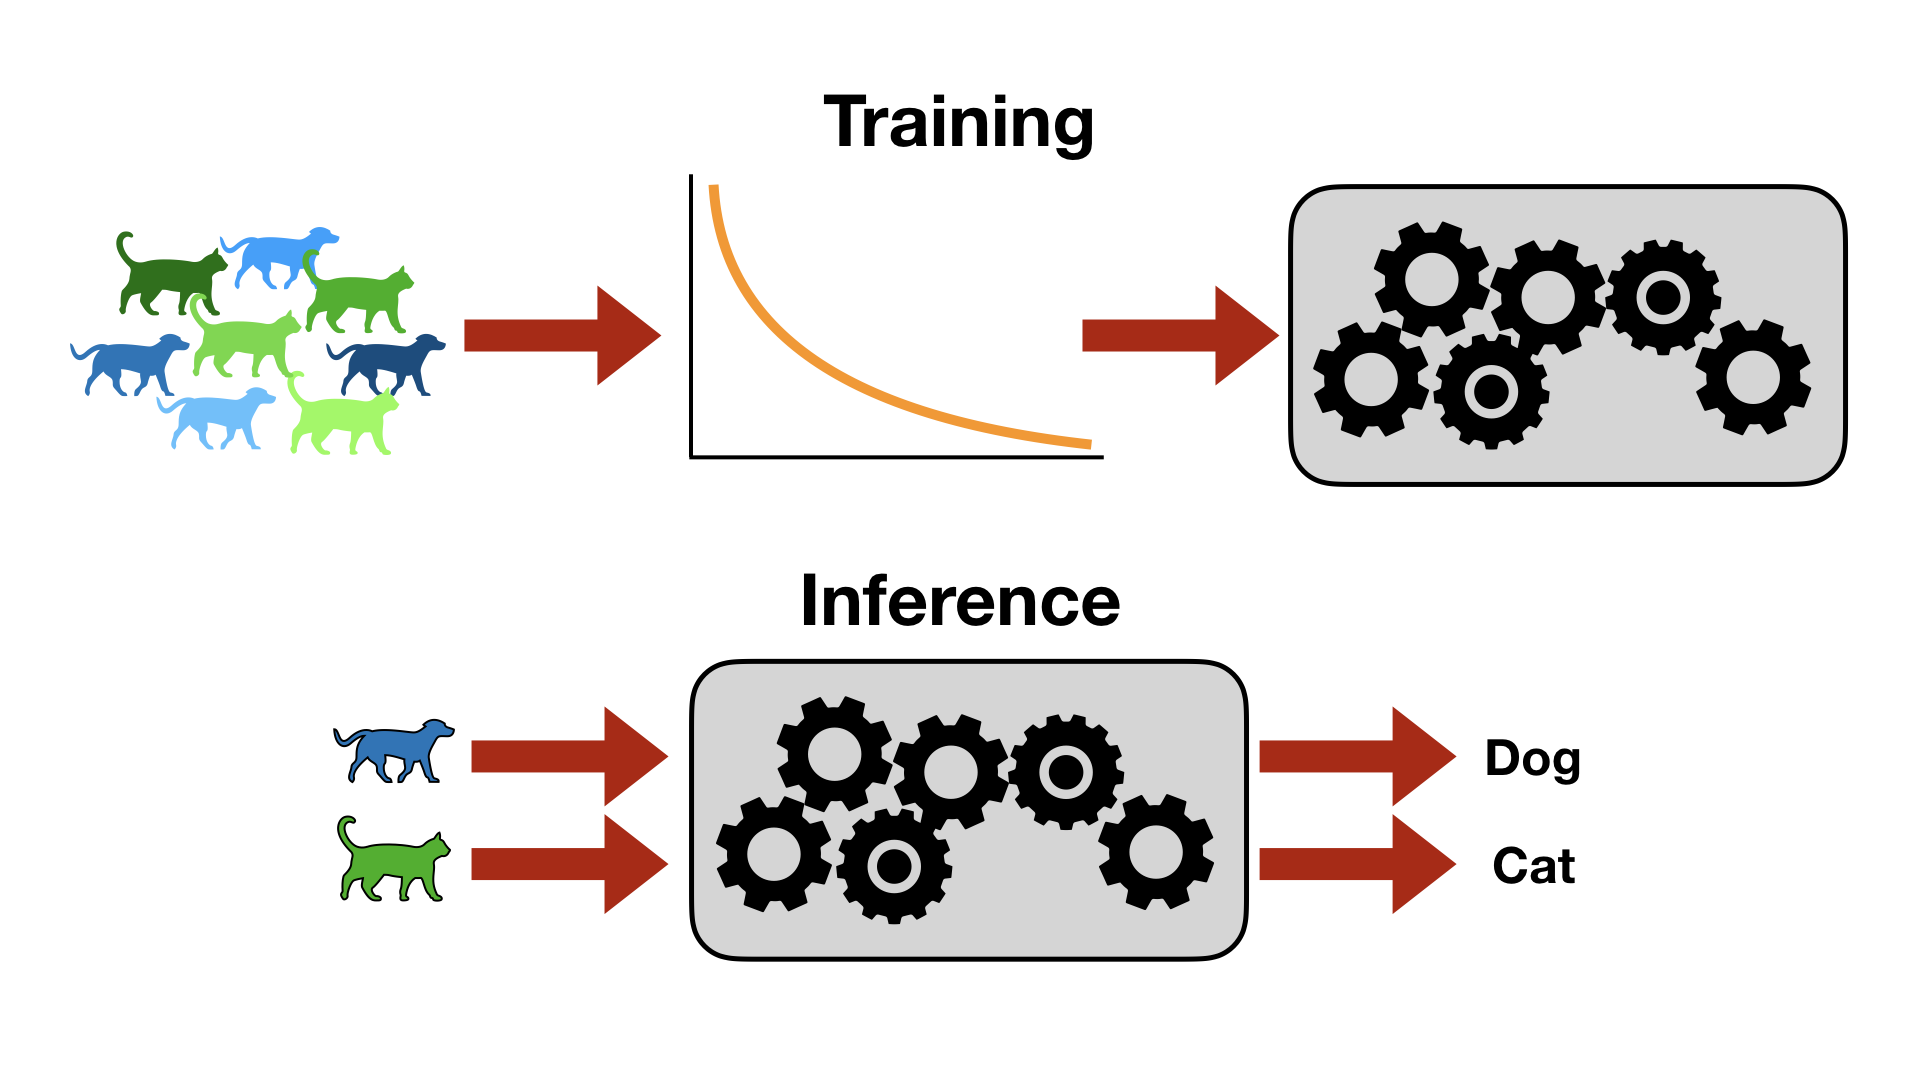
\includegraphics[trim={0 3cm 0 3cm},clip,width=0.95\textwidth]{1_intro/figs/dl.png}
    \caption[Modern machine learning pipelines]{Machine learning training and inference visualization.}
    \label{fig:dl}
\end{figure}

% \textit{Explainability} can be seen as identifying important features of the input, as well as parts of the model (parameters) that ``light up`` for that input. \textit{Fairness} can be evaluated via measures over subsets of the data that correspond to specific groups. 
\newpage
\begin{mdframed}[style=MyFrame]
\em 
\textbf{This thesis} focuses its main efforts on identifying these important subsets of model, feature, and sample space, to enable answering questions necessary for mainstream adoption of machine learning methods.
\end{mdframed}

% In this dissertation, we explore the sizes of these models, samples, and datasets, and 
% analyze under what situations 
% a smaller \textit{subset} of them may be sufficient or important
% for questions that run parallel to standard performance and accuracy measures.

Let us step a bit deeper into a basic illustrative example. In order to ease understanding, we can first begin with a basic formulation of learning methods, from which the questions above can take specific forms. 
Learning methods typically  try to identify a function mapping (model) that is able to complete a specific task at some high level of proficiency. 
% In Figure~\ref{fig:dl}, a model is trained using examples of classification task (top), in order to accurately predict the class of a newly provided input (bottom).
% \begin{figure}
%     \centering
%     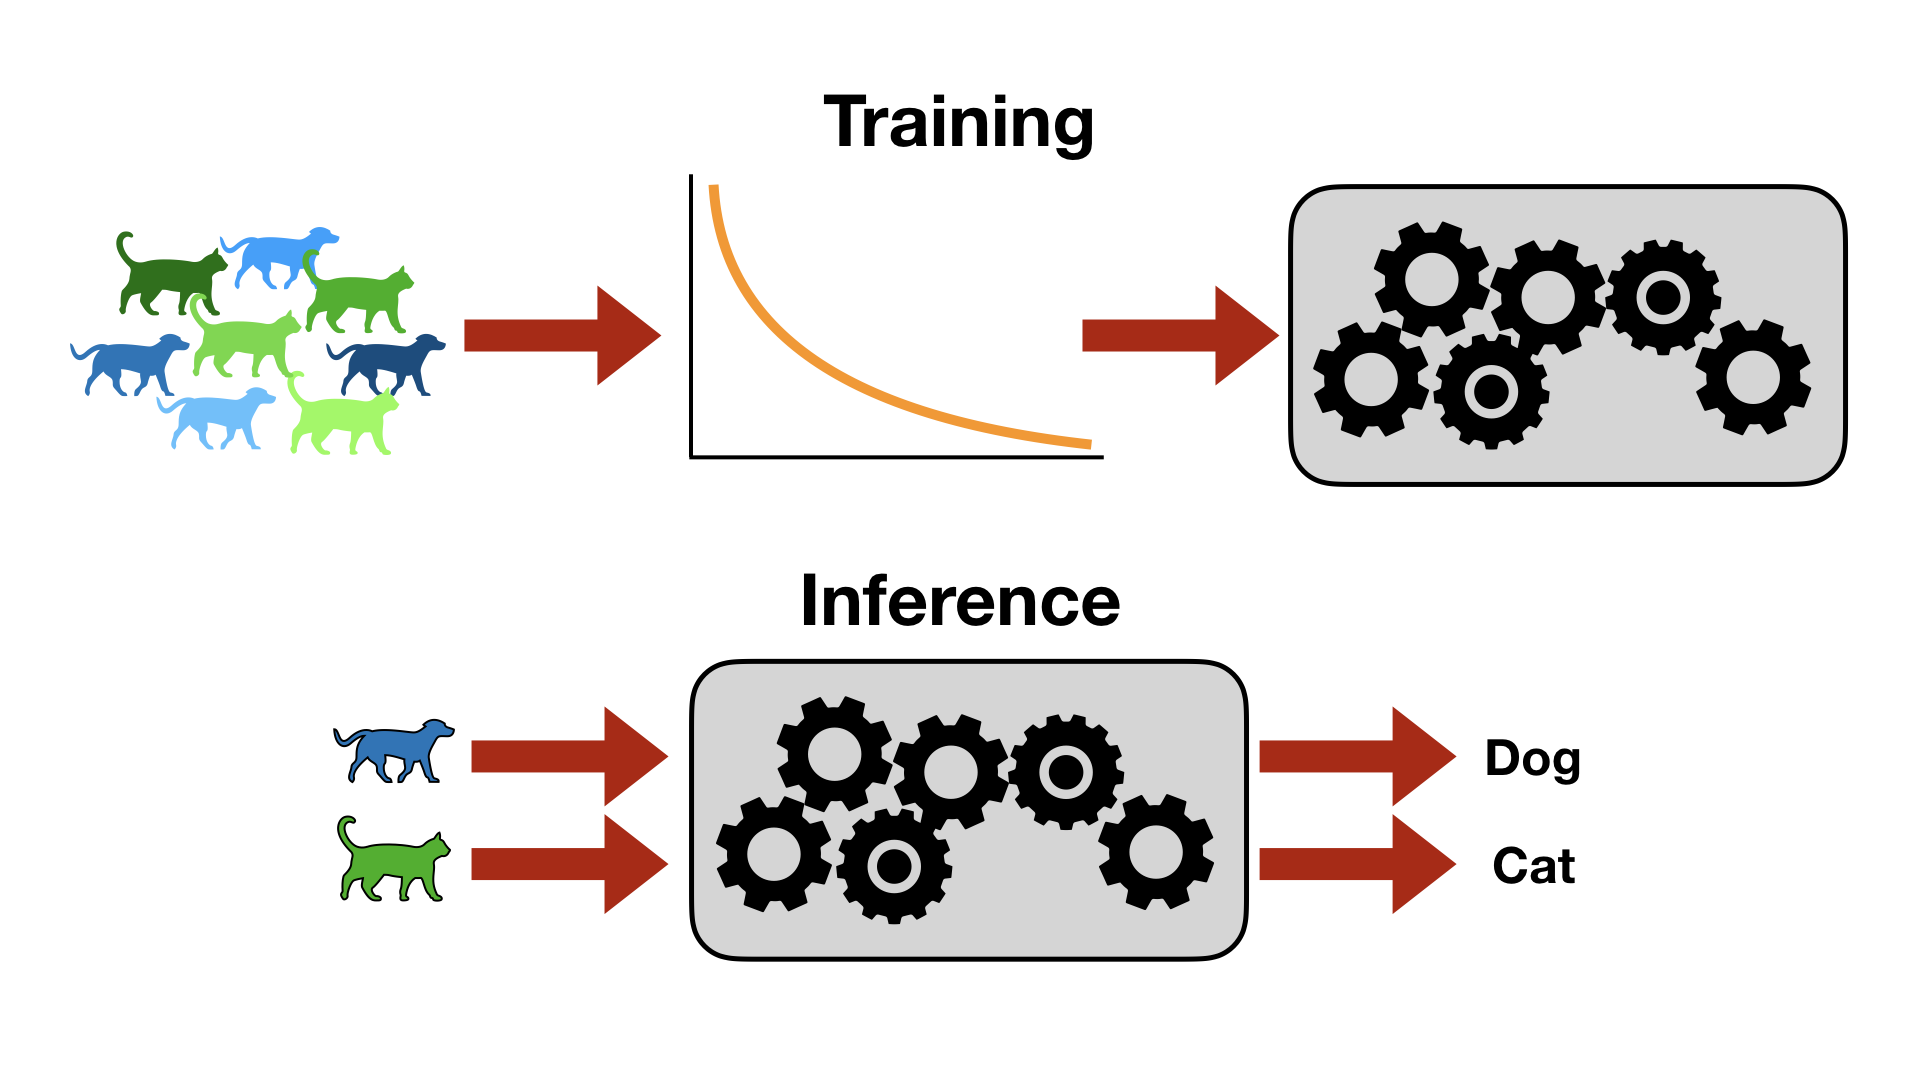
\includegraphics[trim={0 3cm 0 3cm},clip,width=0.95\textwidth]{1_intro/figs/dl.png}
%     \caption[Modern machine learning pipelines]{Machine learning training and inference visualization.}
%     \label{fig:dl}
% \end{figure}
Say we have some dataset comprising of sample pairs $(x,y)$, where we wish to predict $y$ from $x$.
Our prediction, say $\hat{y}$, might be the output of some unknown function $f$ that we attempt to learn from training data. 
Let our approximation to this function be $\hat{f}$.
This can take many forms, 
based on assumptions and prior information we may have on the relationships among the data. 
Consider the simple \textit{linear} case,
where we want to learn some parameter $w$ such that $y = w\cdot x$. 
Given $n$ sample pairs $(x_i,y_i)$ indexed by $i$, traditional statistics and optimization literature yields the following \textit{least squares} problem formulation, where we want to minimize the ``squared error'' between the observed values $y_i$ and the predicted $\hat{y}_i:= w\cdot x_i$:
\begin{align}\label{eq:lq}
\hat{f}:=\hat{w} = \mathop{\arg\min}_{w} \sum_{i=1}^n (y_i - w\cdot x_i)^2
\end{align}
This formulation extends without much change to a multi-dimensional form of the input $x$ and respectively, $w$: the canonical case where a number of features, say $d$, of $x$, or \textit{covariates} (e.g., symptoms), are used together to predict the outcome (e.g., diagnosis). 
This is typically represented as a $d$-dimensional vector, with
each position representing a different feature.
If we are interested in which features of $x$ are important, we can look at the relative values of the learned ``weights'' $w$. In this simple setting, the importance of a feature (say $x^j$) can be exactly determined by the importance of the parameter ($w^j$).
A weight value far from zero may indicate that corresponding feature is important for diagnosis.
% If instead we are interested in which samples are most important, we can use existing methods for sample reweighting or methods that use standard assumptions to efficiently identify important subsets.

In this case and others, traditional statistical learning methods 
have been studied 
for many decades.
Linear regressors, decision trees, and support vector machines
have all been analyzed under this lens.
% ,
% and as the modern machine learning community
% has returned to these questions recently,
% so has a renewed interest in their methods of analysis.
New research focuses
particularly on the differences
associated with moving from classical \textit{under-parameterized} models to
modern (deep) \textbf{over-parameterized} models: where
the model size vastly outnumbers the number
of input samples.
% , and may even be comparable to 
% the \textit{entire sample space.}
Methods for estimating the number of samples needed,
the time to learn a particular task,
and the generalization ability 
all require new perspectives in this regime.
While nascent, these high-dimensional approaches
attempt to fill the gap between
statistical and deep models to enable similar measures of sample influence, feature importance, and model understanding. 

\paragraph{A full picture.}
Let us expand our notation from the example above to consider this more general framing.
Consider a dataset $X:=\{x_i\}_{i=1}^n$ of size $n$ where each data point $x_i$ in the set $X$ is drawn from some underlying distribution over the domain $x_i \sim \cX^d$, 
with domain dimensionality (number of features) $d$ (typically indexed by $j$ as $x^j$).
A model $f$ is fit using a parameterization $\theta \in \Theta$,
with $\Theta$ the space of possible parameterizations (models) with some intrinsic dimension $p$. 
%While all three of these problems are closely related, they require different approaches. 
Generalizing the least squares ``error measure'' from~\eqref{eq:lq} to an arbitrary \textit{loss} $\ell$, we have
\begin{align}\label{eq:learning}
    \hat{f}:=\hat{\theta} = \mathop{\arg\min}_{\theta\in\Theta} \sum_{x_i \in X} \ell(f_\theta(x_i))
\end{align}
From an analysis perspective, 
we might be interested in any one of 
\textbf{(a)} subsets of input features $\cF \subseteq \cX$ that are important for the downstream task,
\textbf{(b)} associating model subsets $\cP \subseteq \Theta$ with specific inputs or groups of inputs, or 
\textbf{(c)} subsets or subgroups of samples $S \subseteq \{X\}$ that are sufficient or representative of the entire dataset.

Crucially, an uninformed search for a subset is computationally infeasible. For a superset of size $n=|X|$, the set of all subsets is the power set, with a size of $2^{n}$! If an identification procedure requires looking over all of these and choosing a ``best'' one by some measure, the procedure will be limited to very small supersets.
Efficient methods have been developed in each of the three contexts above to avoid this exponential search.

\begin{figure}
    \centering
    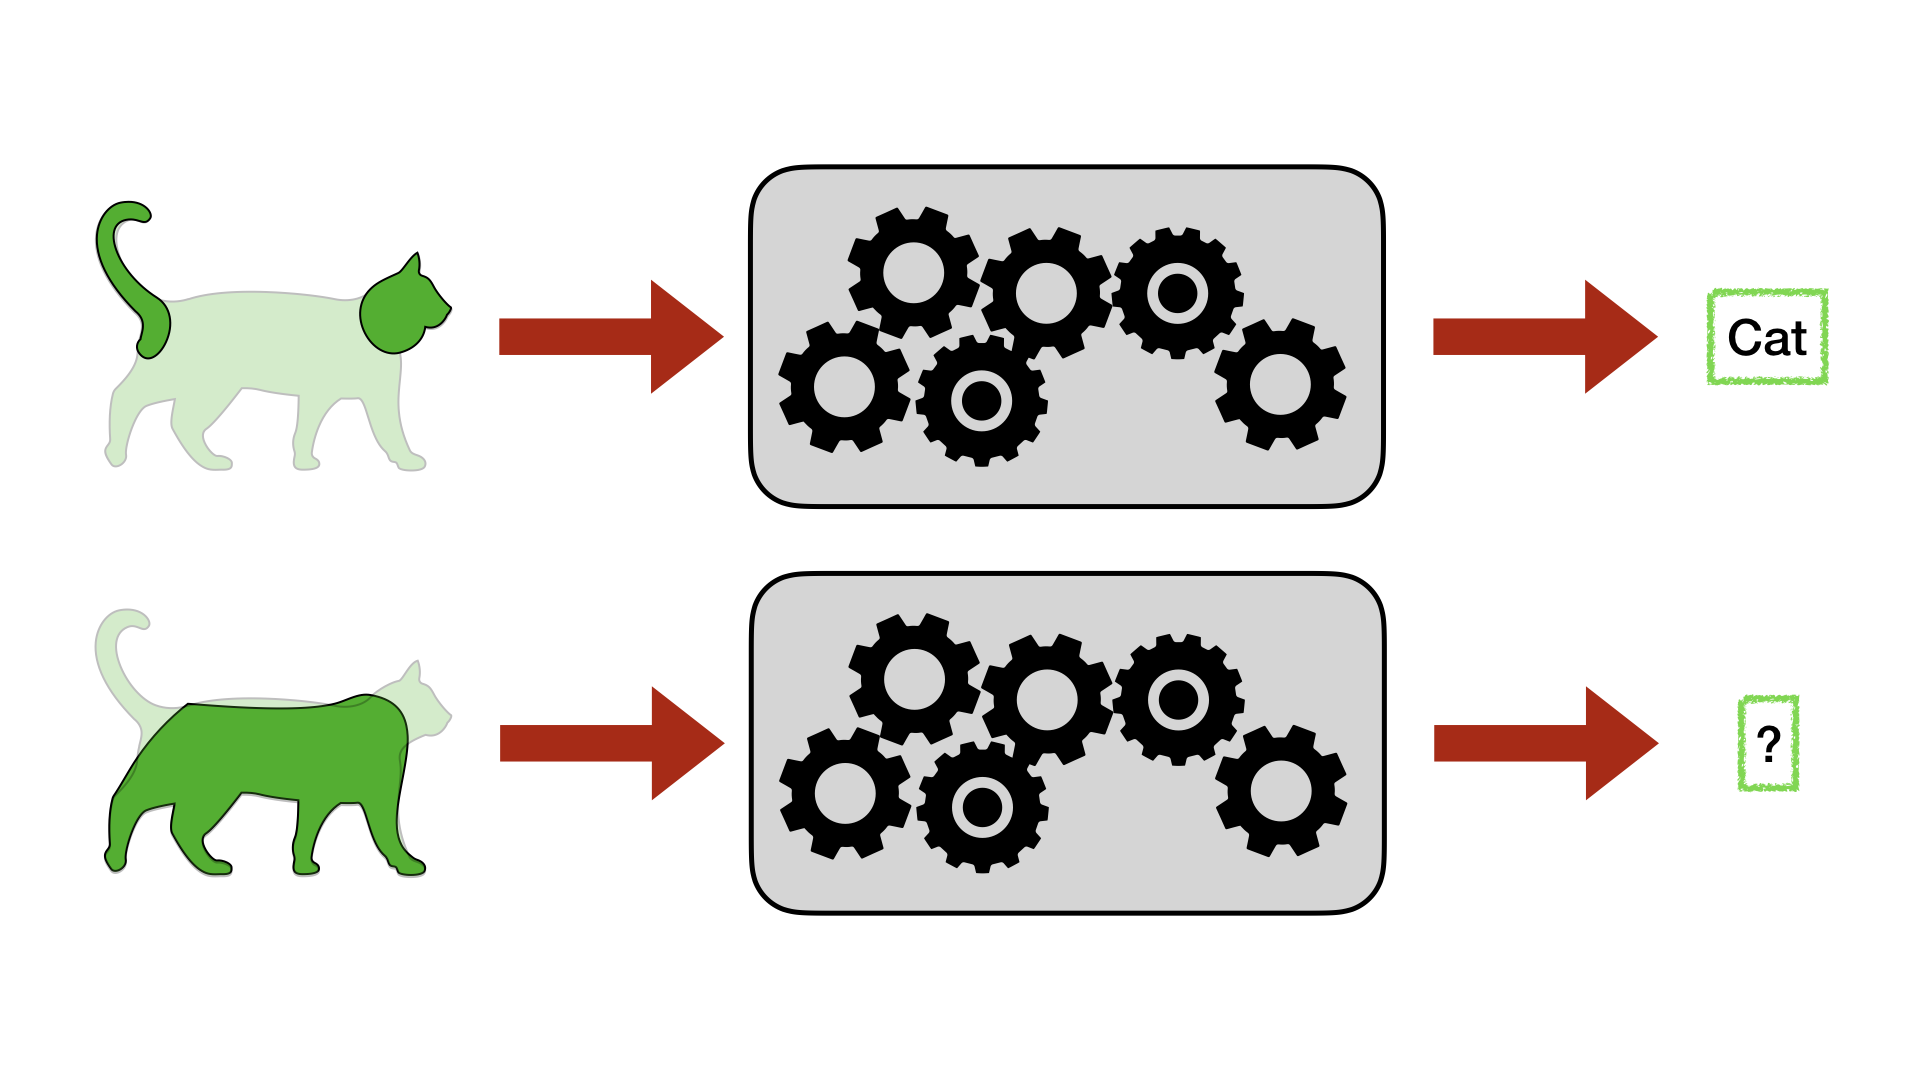
\includegraphics[trim={0 3cm 0 3cm},clip,width=0.9\textwidth]{1_intro/figs/feat_select.png}
    \caption[Visualization of feature selection]{An example of identifying specific features important to the learning task.}
    \label{fig:feat_select}
\end{figure}
\paragraph{Feature Selection.} 
From the statistics side,
penalized weighting of parameters in models similar to Equation \eqref{eq:lq} has been
analyzed thoroughly, proving effective \textit{sparse} recoveries, with
nonzero elements identifying the selected features.
Correlation and other statistical measures such as mutual information can be used to 
identify features that relate most to the outcome of interest
based on the chosen measure.
Analyses of variance and covariance
have been widely used to determine 
if statistically significant relationships
among variables of interest.
When the number of variables is large,
but an assumption can be made about their
internal structure,
scan statistics~\citep{scanstat,scanstatlrt} allow for a structured ``scanning'' over the input space, skipping subsets of features unlikely to demonstrate relationships based on the measure of interest.
Adaptations of sensitivity analysis, via noise addition and perturbations have found success~\citep{yeung2010sensitivity,zhang2015sensitivity}, alongside activation mapping~\citep{cam,selvaraju2017grad}.
These methods typically generate an analagous ``weighting'' over the input space, identifying features most salient for the specific task (Figure~\ref{fig:feat_select}).

These weighting approaches work well with more complex models $f$ compared to the linear case above: newer ``black-box'' methods have been developed for identifying important features.
Recent popular methods with broad applicability include SHAP (Shapley Additive Explanations) and LIME (Local Interpretable Model-agnostic Explanations)~\cite{shap,lime}.
Shapley methods estimate the importance, or weight, of a particular feature for a prediction through randomized masking to estimate marginal contributions.
LIME samples the model space around the input of interest to estimate the decision function locally, penalizing complexity of this estimation to enable interpretability of the explanations.
Predominantly created and deployed in computer vision and imaging domains, these methods have proven effective in identifying parts of the input that drive the function output.
In models that generalize well, these features correspond to regions of the image that a human would use in performing the same task.


\begin{figure}
    \centering
    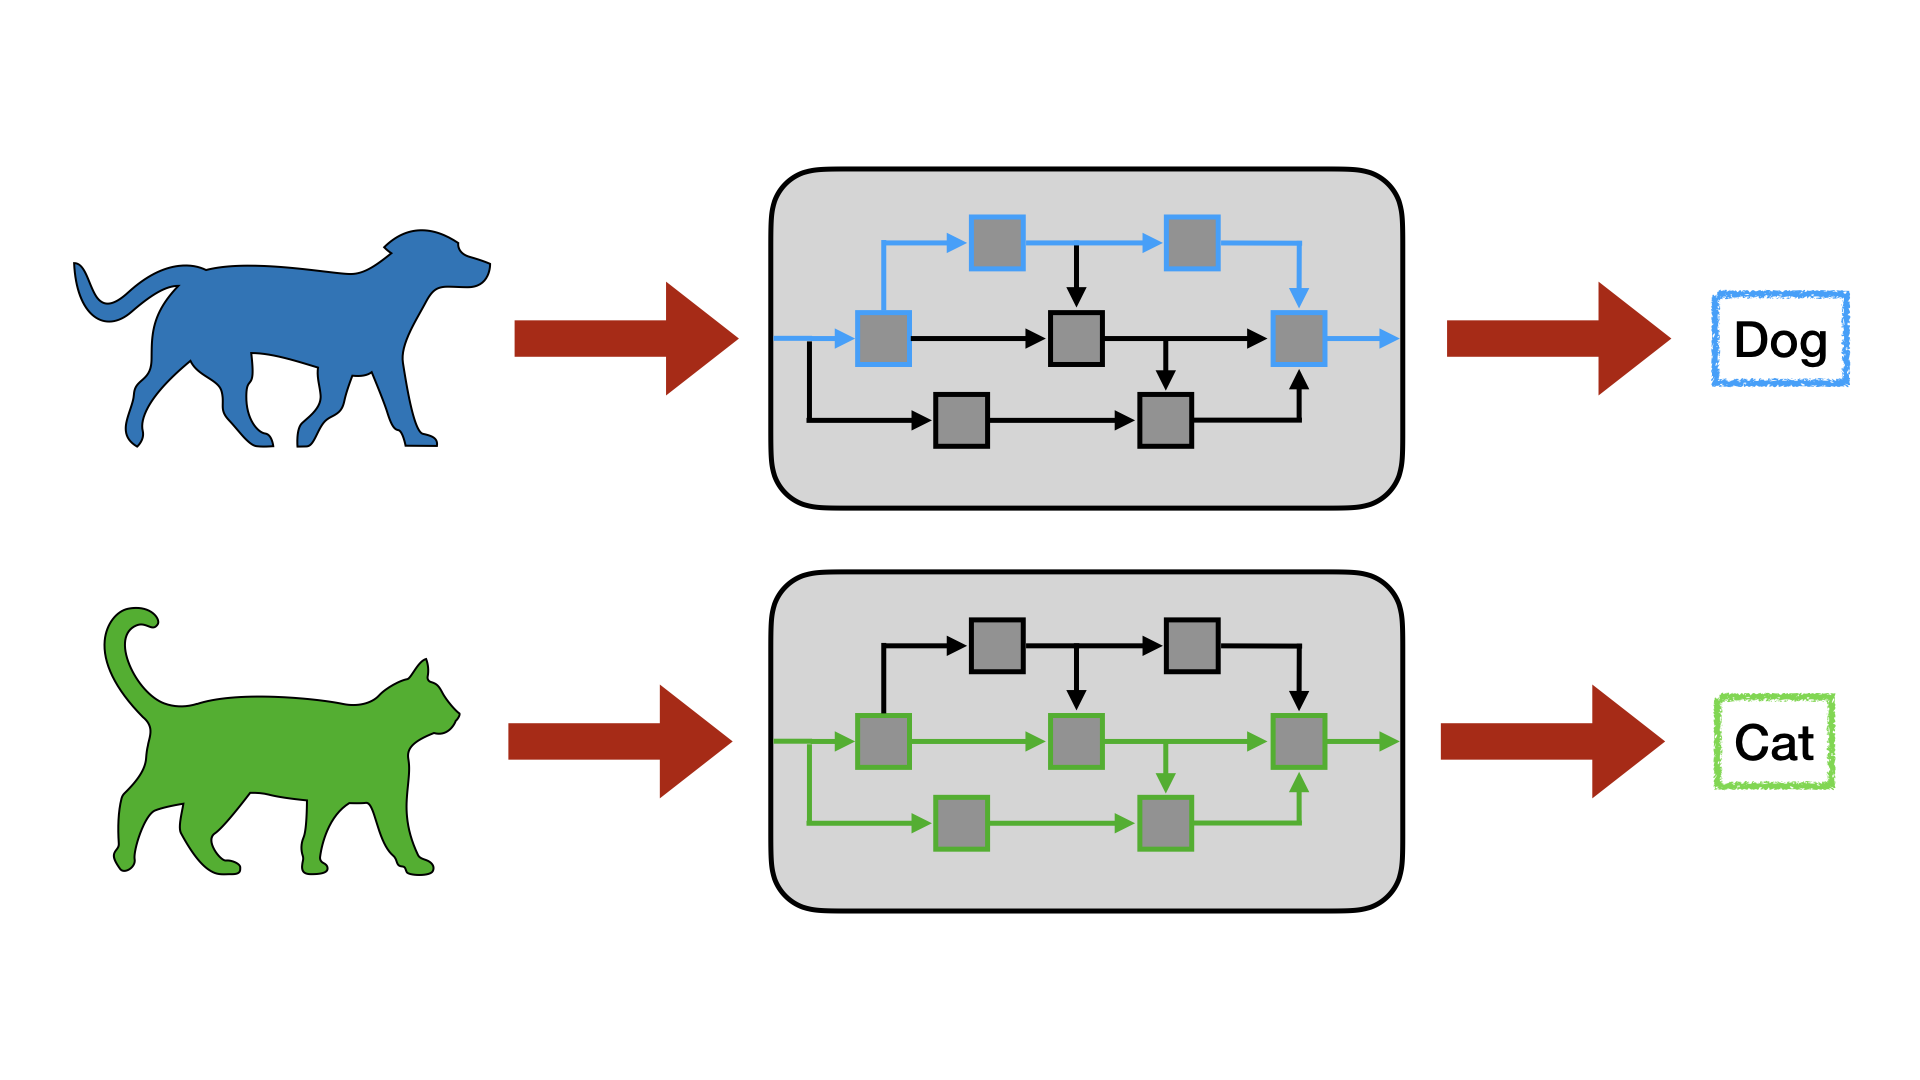
\includegraphics[trim={0 3cm 0 3cm},clip,width=0.9\textwidth]{1_intro/figs/param_select.png}
    \caption[Visualization of parameter selection]{An example of identifying specific parameters important to the learning task.}
    \label{fig:param_select}
\end{figure}
\paragraph{Parameter Selection.} 
Selection in the model space generally takes two forms. First, as a prior, restriction, or assumption over the model space, and second, as a post-hoc method for an ``explainable'' proxy.
Regularization, sparsity, and gating methods are often used independent of the type or size of the model, to encourage the solution to fall within a specific region of the model space.
% In non-deep settings these methods come with strong theoretical guarantees. 
A complete picture of the theoretical underpinnings of these methods in deep learning has not yet been identified, but some progress has nonetheless explained their effectiveness in practice~\citep{hardt2016train,jacot2018neural,neyshabur2014search}.
Outside of the actual training process,
a number of methods have been proposed for \textit{model} selection.
By far the most valuable approach in scalable machine learning has been architecture search, enabling a higher-level identification of \textit{which} parameters should be learned, and what their relationship should be~\citep{elsken2019neural}.
With a model learned, identifying a simpler model takes the form of \textit{knowledge distillation}.
Originally presented in~\cite{hintondistill} and overviewed for modern DNNs in~\cite{gou2021knowledge}, the technique involves training a simpler ``student'' model to mimic the output of the original, complex ``teacher'' model.
To aid interpretability, \textit{disentanglement} approaches have been widely successful,
with the goal of associated specific, distinct, parameters or regions of model space with salient factors of variation within the data~\citep{creager2019flexibly,locatello2019challenging}.
Text and image generation models have benefited largely from similar ideas, enabling tunable ``knobs'' corresponding to independent features of interest~\citep{higgins2017betavae,karras2019style,hjelm2018learning}.

Of particular interest here are the parameters relevant to specific regions of the input space \textit{after} training (Figure~\ref{fig:param_select}). 
Here, recent analysis of deployed networks has shown that indeed, models tend to learn subsets of parameters corresponding to specific subregions of the input space, or subtasks~\citep{bau2017network,fong2018net2vec}, and current work continues to explore these network regions to aid in interpretability and explainability~\citep{netdissect,yiyou}, some associating specific paths through the network with specific tasks~\citep{geigerinducing,elhage2021mathematical}.


\paragraph{Sample Selection.}
Interest in identification of a specific sample within the training set, or a sample at test time, 
have led to a number of other approaches.
Identification in the most classical sense takes the form of outlier detection.
Traditional statistics would use some form of the largest error to the model fit,
perhaps after removing that sample and refitting.
In the deep learning setting, we do not have the luxury of 
being able to train a new model for each sample we wish to evaluate.
Thus methods for black-box outlier detection have been developed~\citep{huang2020feature,ren2019likelihood}.
Outliers within the data and embedding space notwithstanding,
the \textit{influence} of a particular sample on learning is of independent interest:
are some samples particularly valuable or detrimental to training?
Is there a minimal set sufficient for learning the task?
Building on ideas in archetypal analysis~\citep{cutler1994archetypal} and coreset identification~\citep{agarwal2005geometric,ravi2019deterministic},
post-training methods have also been effective in understanding
sample influence~\citep{koh2017understanding,golatkar2020eternal,huang2020feature}.

Additionally, once a sample or set of samples has been identified,
it may be the case that we wish to adjust
our model to either increase or decrease their influence or some other measure.
In the context of fairness, a subset of samples may be ``outliers'', but
represent a true mode of the sample space that has not been fit properly.
Then we may want ``in-the-loop'' methods that can adjust
for this individual or group unfairness (``outlierness'') during training~\citep{mehrabi2021survey}.
After a model has been trained however, post-hoc adjustments are difficult.
One topical application of this is machine \textit{unlearning},
where we wish to remove a sample's influence completely without retraining~\citep{bourtoule2021machine,cao2015towards}.
As we will see, this is still yet impractical with existing methods,
and we will use novel tools to construct practical algorithms
for efficient post-hoc model updates based on a sample's influence.

%Many methods have been developed for outlier detection within training or testing sets~\citep{huang2020feature,ren2019likelihood} \textit{after} training, as well as methods for understanding sample influence~\citep{koh2017understanding,golatkar2020eternal,huang2020feature}. ``In-the-loop'' methods for accounting for ``outlierness'' behave similarly to accounting for group or individual fairness while training~\citep{mehrabi2021survey}. Unfortunately, once samples are identified in some manner, post-hoc adjustments to a trained model are generally very difficult. Recent work has focused on ``unlearning'', or removing a sample's influence on a model without retraining. If specific samples can be uniquely identified, performance and privacy reasons may require these specific interventions to reduce the ``influence'' of that sample subset.
\begin{figure}
    \centering
    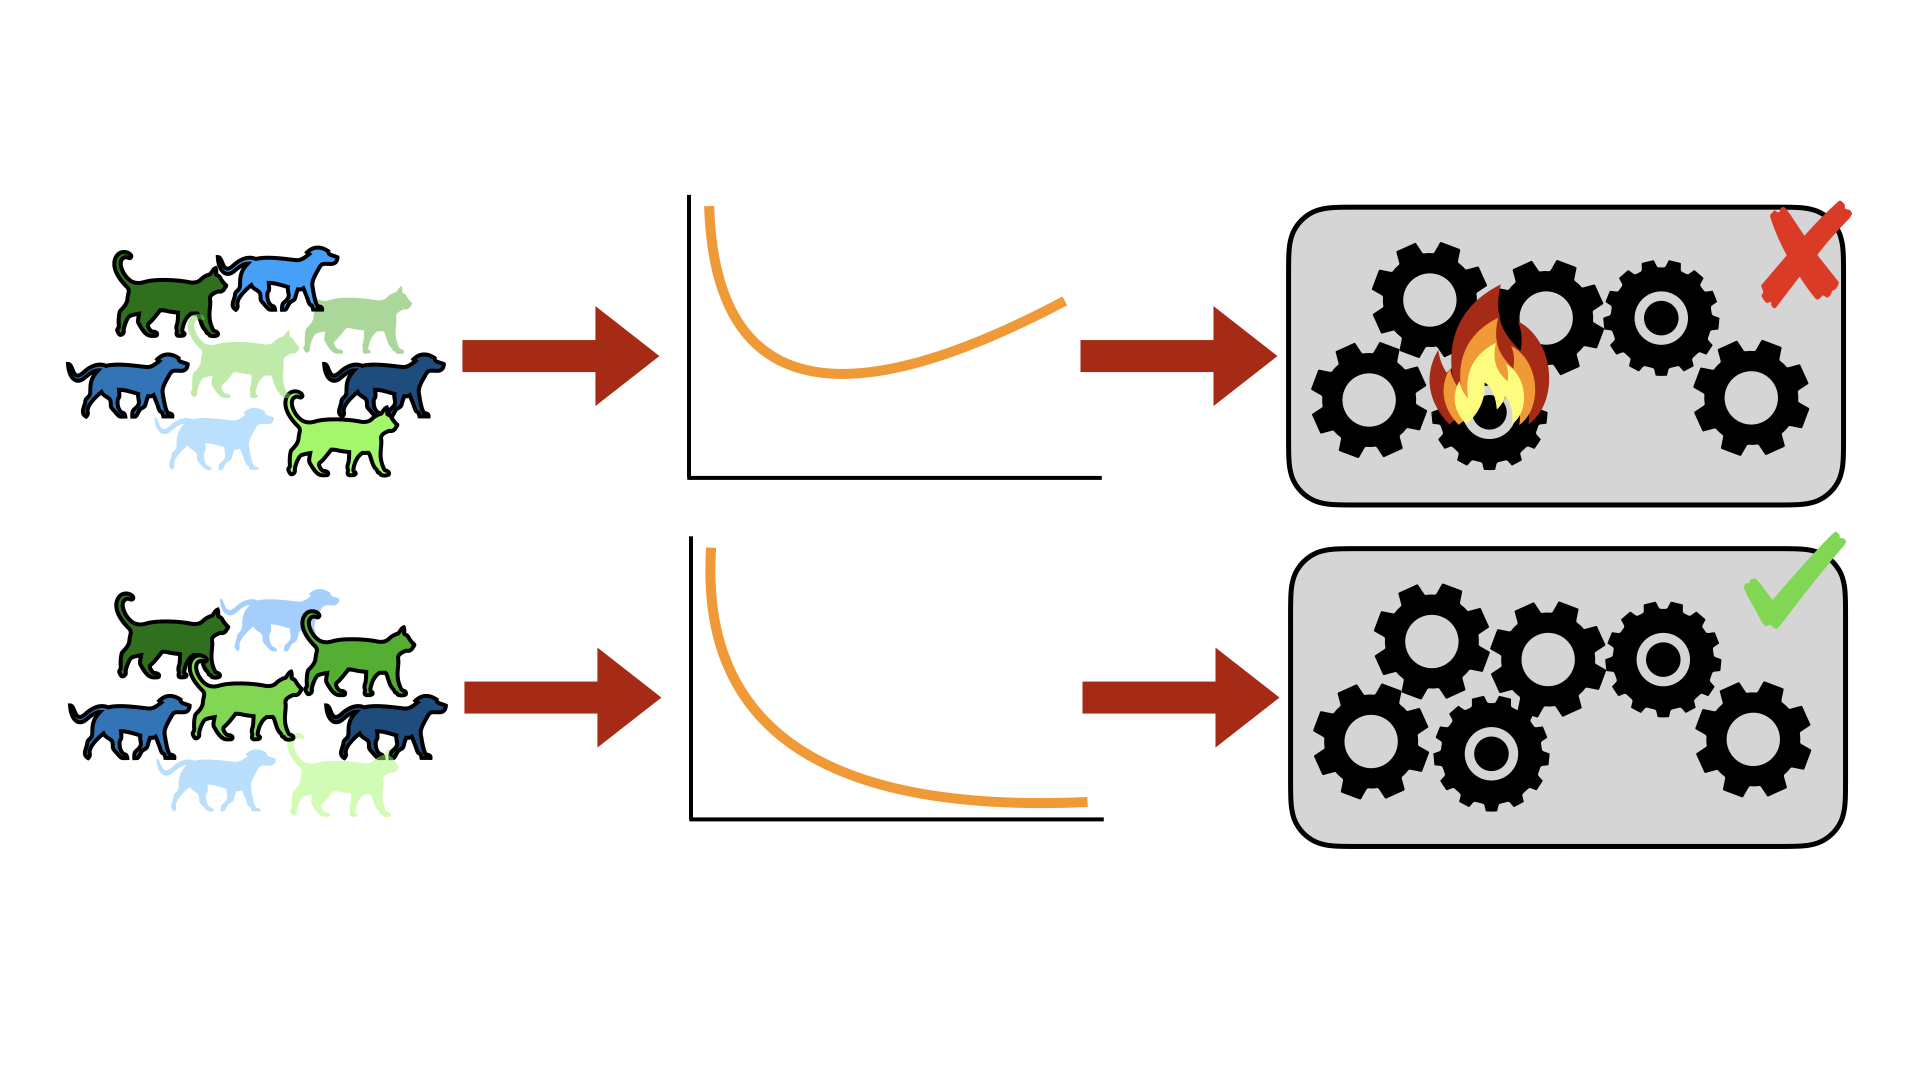
\includegraphics[trim={0 4.5cm 0 4cm},clip,width=0.9\textwidth]{1_intro/figs/sample_select.png}
    \caption[Visualization of sample selection]{An example of identifying specific samples important to the learning task.}
    \label{fig:sample_select}
\end{figure}

\begin{mdframed}[style=MyFrame]
\textbf{ Thesis Goal: }
\em Identify, construct, and evaluate methods for \textbf{efficient} subset identification in modern machine learning feature, model, and input spaces.
\end{mdframed}

\section{A Few Motivating Examples}
Consider a traditional machine learning classification task in which we would like to predict whether an individual has a specific disease condition based on a medical resonance image (MRI) scan of their brain. Our input feature $x$ may consist of a 3D-array of values in $\RR^{\cI\times \cJ\times \cK}$ measuring some intensity of the imaging modality at each voxel, indexed by a tuple $(i,j,k) \in (\cI,\cJ,\cK)$.
Our outcome variable $y$ may simply be a binary label of whether the input scan has been labeled by a radiologist as one demonstrating typical disease characteristics.
Using an off the shelf 3D convolutional neural network with adjustments to match our input size, we can very quickly set up and train a system to predict disease presence with a high degree of accuracy.

\paragraph{Example 1.}
With a prediction for a specific scan, or predictions over a number of scans, we might be interested in identifying which regions of the brain are most important for diagnosis. These regions, $R \subset \cR:=\RR^{\cI\times \cJ\times \cK}$, can be specific groups of pixels in the image that may correspond to known functional networks. Methods such as attention and class activation maps may work here, but there are a few issues. The number of samples available to learn a model is very small compared to the both the dimension of the input and the number of parameters in the model, i.e., $n \ll p$ and $n \ll d$. Thus it is very easy to overfit, and for areas of interest to be associated with intricacies of particular input data rather than true, real differences defined by the disease.

Furthermore, recent medical imaging studies have moved past simple difference detection: trends over time, and the ability to predict {\em future} disease development have by far become the setting of most interest.
Given an image of a healthy individual, is it possible to predict what their scan, or their future disease diagnosis, may be up to 10, 20, or more years in the future?
If a number of scans have been collected over some timeframe, can the \textit{trajectory} of the individuals' development be extrapolated to estimate progression?
As traditional models extended for temporal analysis grow in both size and complexity,
a number of subproblems explicitly related to model and input subspaces arise. In this thesis we address two such problems: \textbf{statistically rigorous identification of temporally evolving subsets}, and \textbf{characterizations of deep models that enable efficient training of recurrent models with large scale time-varying data}.
    
\paragraph{Example 2.}
With the rapid growth of AI and machine learning applications has come valid concerns regarding both guarantees of privacy.
Recent technology legislation has made the importance clear in all aspects of data use,
and particular projects and groups have demonstrated that machine learning is not independent of
this need \citep{Exposing}.
A new issue raised within this intersection is the ``right to be forgotten".
If a model has been trained with a particular users' data, 
they should have some recourse or right
to both remove their data from the training set,
and also know that the model has not learned from their data.
On the surface, this poses a significant problem for model builders
and organizations that spend large amounts
of time and resources in 
training deep learning models.

In the medical imaging example above this is especially important: with fewer samples it is more likely that information about any particular one could ``leak'', and the model's performance may degrade significantly as a relatively large percentage of it's training data is removed.
Thus tailored methods must be developed to ensure both privacy and performance, without requiring full retraining.
As we will see, 
\textbf{identification of model parameter subsets}
that are particularly important
for a particular sample's influence
in a model enables \textit{efficient machine unlearning}.

\paragraph{Example 3.}
From an alternative perspective, we may want to identify specific samples rather than have them specified a priori.
Traditionally a rigorous area of study under classical statistics, outlier detection and accounting have become a subfocus for many within the machine learning community as well \citep{golatkar2020eternal,golatkar2020forgetting,huang2020feature,ren2019likelihood}.
While subgroups of input samples may be outliers, it is more often the case that they represent known heterogeneity within the data. 
These differences may be marked using 
group information known a priori, and 
most learning tasks aim to learn tasks
in a \textit{subgroup-independent} manner.
In our disease prediction model above,
these groups could simply be stratified by the type of scanner used to acquire the image, but it could also
be a systematic difference correlated with some protected or delineating attribute.
Commonly used atlases for brain MRI registration are often constructed
from the scans of predominantly right-handed middle-aged adults~\citep{FONOV2009S102}.
Resulting downstream analysis may be significantly worse
for people outside that age range or those who are left-handed.
These types of biases can directly lead to disparate performance and results on \textit{all} individuals outside of that group.
Optimization and regularization methods with this focus come under the umbrellas of model fairness, enforcing invariance, and spurious feature regularization among others.
However, many existing methods do not scale well to larger models or as the number of subgroups grows,
as is often the case when intersections of protected classes must be considered.
Here we identify and construct a particular solution for \textbf{groupwise fairness that enables efficient in the loop fairness regularization}.

% What features are most important for prediction?
% Which samples were most important for my training?
% Can we understand when a model is certain or uncertain about its output?
% Are there layers in my network that have learned a particular subtask?
% Questions of robustness, bias, influence, fairness, and importance have become central questions to contemporary machine learning research \citep{doshi2017towards,mehrabi2021survey,amodei2016concrete}.
% machine learning, etc.

% Feature selection in the case of
% typical regression or classification 
% takes some form of learning parameters $\theta$ that allow for $\hat{y} = f_\theta(x)$ to be close to the true outcome of interest $y$.
% While forms of data $X := (x,y)$ may simply be continuous and real-valued, modern machine learning has greatly expanded formulations of the classical learning problem to include a wide variety of structured learning problems~\citep{nowozin2011structured}. 
% Consider the case when a high-dimensional input is used to predict an output with a highly-parametrized model. 
% Once learned, obvious questions arise as discussed above: are there specific low-dimensional spaces in either the input or the model space that are most important or necessary for the global learning problem of interest? Are there specific subspaces associated with particular subproblems of the global problem?
% The machine learning literature has come up with a number of ways to identify analogs of these spaces, 
% including extensions of sensitivity analysis to deep learning~\citep{yeung2010sensitivity,zhang2015sensitivity}, and constructing and identifying nonzero model subsets via particular model choices such as activations~\citep{selvaraju2017grad} and regularizers.
% In classical settings these are well understood: decision trees naturally provide ease of interpretibility via the information used to choose splits, and both linear and kernel support vector machines have been analyzed to provide for measures of sample importance via distances to the margin as well as feature importance via weights defining the learned hyperplane~\citep{Mitchell97}.
% Attention and saliency maps have emerged as popular new methods,
% given their ease of implementation and interpretation~\citep{sutskever2014sequence,vaswani2017attention,selvaraju2017grad}.
% By learning dimensions of a given input that are particularly important, either in a hard (binary) or soft (continuous weighting) manner, model builders are better able to understand and interpret what a model has learnt.
% The specific ideas of attention notwithstanding, many of these existing methods are far removed from traditional hypothesis testing frameworks.
% While some work has begun in this direction~\citep{tansey2018black},
% there remains a gap in direct identification of subsets and structures in these spaces that can be defined in statistically rigorous manners.

% \begin{figure}
%     \centering
%     \includegraphics[width=0.5\textwidth]{example-image-a}
%     \caption[A simple subset selection example]{\color{red} Identifying and selecting in MRIs, subset, sample, model ID.}
% \end{figure}

% \paragraph{A specific example.} 

% ------------------------------------------

% below here will be moved and arranged with the "selection" sections and here if relevant

% ------------------------------------------

% While attention can be directly applied to the network in order to identify ``hotspots" in the input space relating to the learned classification task, 
% given the high-dimensional nature of the input
% and the relatively small sample size 
% associated with medical imaging data, 
% it is very likely that an area of interest identified
% may be an intricacy of the training samples used rather than truly a region of disease signal.
% Class activation maps (CAMs) may be unclear, and can often associate with image artifacts unrelated to the scientific task~\citep{adebayo2018sanity}.
% Methods of generalization may help to increase confidence in identified regions, but statistical guarantees often remain out of reach.

% Furthermore, most recent problems associated with medical data have moved past simple difference detection: trends over time, and the ability to predict {\em future} disease development has by far become the setting of most interest.
% Given an image of a healthy individual, is it possible to predict what their scan, or their future disease diagnosis, may be up to 10, 20, or more years in the future?
% If a number of scans have been collected over some timeframe, can the \textit{trajectory} of the individuals' development be extrapolated to estimate progression?
% As traditional models extended for temporal analysis grow in both size and complexity,
% a number of subproblems explicitly related to model and input subspaces arise. Here we address two such problems: \textbf{statistically rigorous identification of temporally evolving subsets}, and \textbf{characterizations of deep models that enable efficient training of recurrent models with large scale time-varying data}.

% A sample's particular influence on model parameters aside, the identification of influential samples or subsets of samples more generally is of independent interest. 
% Traditionally a rigorous area of study under classical statistics, outlier detection and accounting have become a subfocus for many within the machine learning community as well \citep{golatkar2020eternal,golatkar2020forgetting,huang2020feature,ren2019likelihood}.
% While subgroups of input samples may be outliers, it is more often the case that they represent known heterogeneity within the data. 
% These differences are typically marked using 
% group information known a priori, and 
% most learning tasks aim to learn tasks
% in a \textit{subgroup-independent} manner.
% Optimization and regularization methods with this focus come under the umbrella of model fairness, and instead of identifying and boosting independences within the model or data, we aim to minimize them.
% However, many existing methods do not scale well as the number of subgroups grows, as is often the case when intersections of protected classes must be considered. In the sequel we identify and construct a particular solution for \textbf{groupwise fairness that enables efficient in the loop fairness regularization}.

\begin{mdframed}[style=MyFrame]
\em 
Here we focus our effort on identifying these important subsets of model, feature, and sample space for feature association, model size reduction, model unlearning, and, fairness. Specifically, taking advantage of both existing statistical and geometric methods, we develop new methods for localizing subsets in a range of settings from hypothesis testing to deep learning.
\end{mdframed}

\section{Thesis Scope and Contributions}

We explore the intersections of classical statistical and geometric constructions with modern machine learning methods. 
Figure~\ref{fig:scope} shows the overall scope projected along three axes: feature, parameter, and sample spaces.
Below we briefly introduce the main problems studied in this thesis.
\begin{figure}[ht]
    \centering
    % \includegraphics[width=0.99\linewidth]{scope.pdf}
    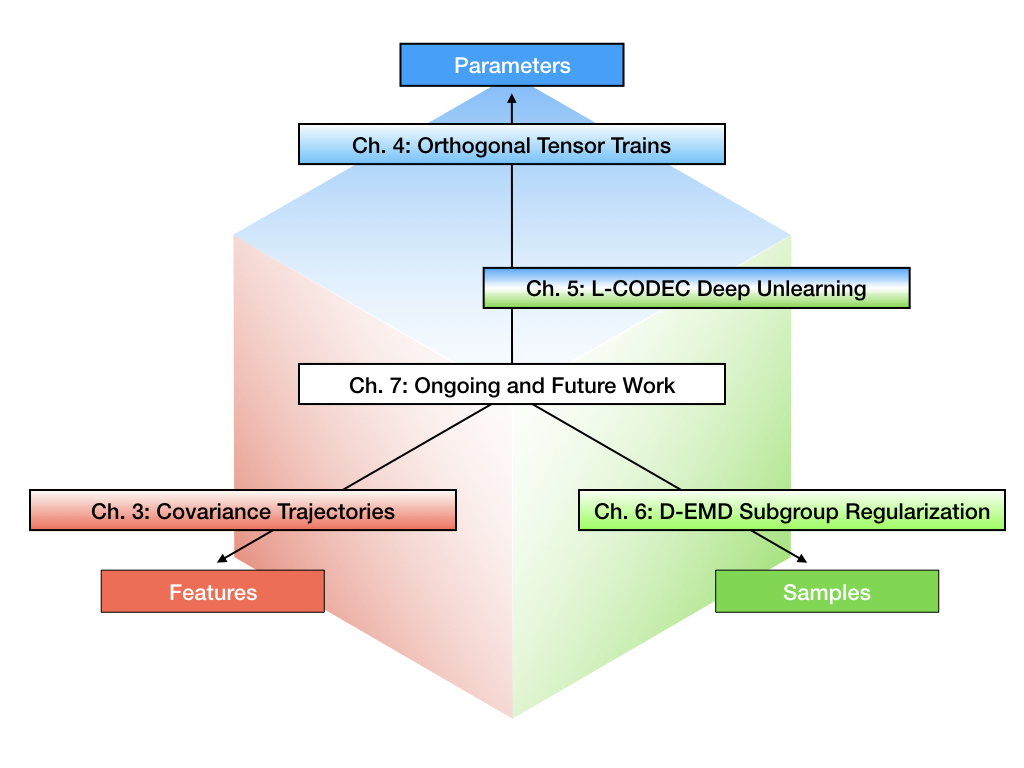
\includegraphics[width=0.95\linewidth]{1_intro/thesis_scope_diss/thesis_scope_diss.png}
    \vspace{-10pt}
    \caption[Thesis scope]{Thesis scope, projected over three representative axes.}
    \label{fig:scope}
\end{figure}

\subsection{Chapter 3: Second-Order Modeling and Group Difference Analysis over Time}

Results in coupled or temporal graphical models offer schemes for estimating the relationship structure 
between features when the data come from
related (but distinct) longitudinal sources~\citep{zhou2010time,caffo}. A novel application of these ideas is for analyzing group-level differences, i.e., in identifying if {\em trends} of estimated objects (e.g., 
covariance or precision matrices) are different across disparate conditions (e.g., gender or disease).
Often, poor effect sizes make detecting the \textit{differential} signal 
over the {\em full} set of features difficult: 
dependencies between only a {\em subset of features} may manifest differently across groups.
%Here we will take a look from the perspective of \textbf{feature subset identification}.
We first suggest
a parametric model 
for estimating trends in the space of $\SPD$ matrices as a function of one or more covariates.
With this in hand,
we move on to using 
graphical model approaches to determine
on which covariates sets it is most meaningful to 
fit these trends.
We generalize scan statistics to graph structures, 
and search over distinct \textbf{subsets of features} (graph partitions) whose temporal dependency structure may show statistically 
significant group-wise differences.
We theoretically analyze the Family Wise Error Rate (FWER) and bounds on Type 1 and Type 2 error. 
On a cohort of individuals with risk factors for Alzheimer's disease (but otherwise cognitively healthy), 
we 
find scientifically interesting 
group differences and associated subsets, where the default analysis, 
i.e., models estimated on the full set of features, do not survive reasonable 
significance thresholds. 
% Preliminary work on this was published in \citep{covtraj}.


\subsection{Chapter 4: Efficient Tensor Representations for Feasible Temporal Deep Learning}

Modern deep networks have proven to be very effective for analyzing real world images.
However, their application in medical imaging has required additional and specific machinery,
primarily due to the large dimension of three-dimensional images,
requiring enormous network architectures --
if we treat an image (and not image patches) as a sample. 
These issues only compound when the focus moves towards longitudinal analysis
through recurrent structures, and when a point estimate of model parameters is insufficient 
in scientific applications where a reliability measure is necessary.
Building upon the differential geometry insights from the previous chapter, 
we will adapt 
a particular tensor decomposition, the tensor train, to construct networks
with significantly fewer parameters.
Using the theoretical guarantees afforded by its 
geometry,
it enables us to train powerful recurrent networks on whole brain image volumes. 
Resembling \textbf{model and parameter selection} methods
such as compression and distillation,
we analyze 
the \textit{orthogonal tensor train},
and demonstrate its ability to represent a standard network layer both theoretically and empirically.
We 
demonstrate its ability to 
effectively reconstruct whole brain volumes
with faster convergence and stronger confidence intervals
compared to the standard tensor train decomposition. 
We provide code and show experiments on the ADNI dataset
using image sequences to regress on a cognition related outcome.
% Preliminary work on this was published in \citep{ott}.

\subsection{Chapter 5: Practical Unlearning via Large-Scale Conditional Independence Testing}

%With AI systems extensively using personal %data for model training, 
Recent legislation has
led to interest in {\em machine unlearning}, i.e., removing specific training samples from a {\em predictive} model as if they never existed in the training dataset. 
Unlearning may also be required due to  corrupted/adversarial data or simply a user's updated privacy requirement.
For models which require no training ($k$-NN), 
simply deleting the closest original sample can be effective. 
%However, it is not clear how such approaches can be used to unlearn 
%models that contain rich information learned from the original data.
But this idea is inapplicable to models which learn richer 
representations.
%from data. 
%Recently, optimization-based unlearning estimators have been proposed, but 5their 
Recent ideas leveraging optimization-based updates
scale poorly with the model dimension $d$,  
due to 
inverting the Hessian of the loss function. %with an overall cost of $O(d^3)$ 
%is prohibitive.
We describe
a variant of a new conditional independence coefficient, 
L-CODEC, to identify a \textbf{subset of the model parameters} with the most semantic overlap on an individual sample level. 
Our approach completely avoids the need to invert a (possibly) huge matrix. 
By utilizing a Markov blanket selection, 
we find
that L-CODEC is also suitable for deep unlearning,
as well as other applications in vision.
Compared to alternatives, L-CODEC makes approximate unlearning possible 
in settings that would otherwise be infeasible, 
including vision models used for face recognition, 
person re-identification 
and NLP models that may require unlearning samples identified for exclusion.
% Preliminary work on this will appear in \citep{lcodec}.


\subsection{Chapter 6: Reducing Subgroup Fairness via High Dimensional Earth Mover's Distances}

Optimal transport has recently emerged as a useful tool 
for machine learning through its connections with geometry,
statistical machine learning, and through practical algorithms.
Existing methods that leverage optimal transport often  regularize using 
a Wasserstein metric or by computing barycenters, for example. %which are effective when distributions are continuous and known, or when measures of interest are discrete.
% Our formulation allows for a discretization of continuous measures that drop in directly to classical  formulations of the Earth Mover's Distance. 
We leverage optimal transport,
except that we take advantage of a recently-introduced algorithm
that computes a generalized earth mover's distance.
Not only is this algorithm computationally cheaper
to compute compared to existing barycentric measures,
but our method has the additional advantage that gradients used for backpropagation 
can be directly read off of the forward pass computation, which leads to substantially faster model training.
This speedup enables practical methods of accounting for large \textbf{subgroups of samples} that
may need to be treated equally when stratified.
We provide technical details about this new regularization term and its properties, 
and 
experimental demonstrations of improved training speed over existing Wasserstein-style methods.

\subsection{Chapter 7: Conclusions and Future Work}
The thesis will conclude
with brief descriptions of 
both completed and ongoing
work that has been strongly motivated
by the methods developed herein.
Chapters \ref{chap:covtraj} and \ref{chap:ott} above have been extended 
in a number of directions,
and continues to influence
future research direction. 
The more recent work in Chapters \ref{chap:codec} and \ref{chap:demd}
is serving as an ongoing foundation
for new work.
Developments include 
developing and providing a plug-and-play efficient optimal transport tool 
for community use,
addressing a important gap in existing off-the-shelf methods.
Particularly motivated by the general shift towards ensuring models such as GPT-2 and Stable Diffusion are fair and equitable,
we conclude with a brief reflection
on the role of conditional independence
as a measure of influence and its role in interpretability.
%vision of how these methods may be more broadly applicable,
%and present some extensions of the conditional dependence tools
%developed above in the analysis of latent spaces in recent large scale models.
%Through large language models like GPT
%and high-fidelity
%image generation models such as Stable Diffusion,
%performance is no longer 
%seen as a practical barrier for generation.
%Focus has shifted to ensuring these models
%are acting in accordance with
%fairness, bias, and regulatory requirements,
%and towards better understanding and interpreting
%their large and dense internal mechanisms.
%We close out the thesis with a brief application 
%of conditional independence measures towards
%explaining and understanding the behavior 
%of these models through their latent spaces.

% In these studies, 
% we aim to identify conditionally independent features and subjects that are particularly important to the prediction and estimation of
% key disease outcomes,
% as a function of a number 
% of demographic, neuropsychological,
% genetic,
% and imaging data collected as 
% part of an ongoing consortium 
% to understand the progression
% of Alzheimer's disease in younger, 
% asymptomatic populations.
% In what follows we present
% exploratory analysis
% on a small, easily 
% digestible subset of the available data,
% that lays the foundation for
% further analysis.
% This work is the most forward looking, and aims to be a stepping stone toward a rigorous 

\section{Outline}
Chapter 2 covers the essential background necessary for the developments presented in the following chapters, including specifics of graphs and hypothesis testing, as well as relevant modern methods for learning and optimization.
In Chapters 3 through 7, we describe four perspectives to address subset identification.
Chapter 3 explores and focuses on the identification of feature subsets varying over time.
In Chapter 4 we describe a method of constraining the parameter space in a particular manner
that enables more efficient large scale neural networks.
Next, Chapter 5 provides a solution to the machine unlearning problem,
enabled through a particular conditional independence parameter selection scheme, vastly reducing network update costs.
Chapter 6 ends with a unique solution to subgroup fairness, 
where we take advantage of an efficient solution to
the $d$-dimensional earth mover's problem
to regularize large models when the number of subgroups can be large.
We conclude in Chapter 7 with ongoing and future work, as well as some final thoughts.
%focused on applying a particular solution from Chapter 5
%to understanding relationships among features
%in latent spaces learned by large generative models.


%%%%%%%%%%%%% 
% Some old stuff

% Significant progress in the modern development of machine learning has
% been built upon connections and patterns identified across myriad
% interdisciplinary fields of study.
% Up through the mid 2000's, 
% many of these methods were inspired by and interested in 
% highly focused and constrained problems. 
% With a reasonably sized input domain, could a model of roughly equal size be used to
% predict some output?
% Linear regressors, decision trees, and support vector machines were all answers to these questions, with their own
% varying degrees of scaling and complexity.
% These methods necessitated carefully constructed formulations with specific restrictions to the learnable function class,
% enabling straightforward analysis 
% for provable performance guarantees 
% and easy identification of critical training samples and important input features.

% Contemporary machine learning, however, has a vastly different modus operandi. 
% Driven in large part by the exponential growth of available computation via Moore's Law, \textit{deep learning} has fallen squarely in the realm of \textbf{over-parameterized} models.
% With these overparametrizations and computation capacity, the typical learning questions posed as maximizing accuracy or reducing error have largely been addressed for even large scale problems.
% As such, complementary questions have led to subfields focusing on other performance measures, such as robustness, fairness, interpretability, and explainability.
% Many solutions to these questions end up looking back at answers found for the under- or non-parametrized settings.
% While nascent, these approaches 
% attempt to fill the gap between
% statistical and deep models to enable similar measures of sample influence, feature importance, and model analysis. 
% Most notable amongst these newer approaches is that of (Self)-Attention in Neural Networks \citep{sutskever2014sequence,vaswani2017attention}.
% Other proposals 
% end up looking back at the types of analysis typical of those more classical under-parametrized or nonparametrized methods.

% Not limited to previous developments in learning or computation theory, the arguably most valuable contributions toward the exponential reduction in model error can be attributed to influences and intuitions taken
% from biology, psychology, neuroscience, and even XXX \citep{srivastava, etc}.
% Perhaps one explanation as to why this phenomenon exists may be attributed to the way in which deep learning evolved. 
% The classical learning goal of function approximation lends itself nicely to a system which allows for arbitrary complexity via simple changes (e.g., addition of neural network layers). % Foundational works building on the original neural networks particularly have taken advantage of constraining this space of functions to search over: 
% the most seminal case being those of convolutional filters for imaging data. 
% While ``constraints" of this form have helped tremendously in model performance on modern vision and language machine learning tasks (GANs, Recurrent Networks, Residual Layers, Transformers, etc.), the ability to identify \textit{subsets} of important samples, input features, and model parameters has lagged significantly behind the development of these methods.
% Recently larger interest has been taken by the community to understand and interpret models with this view, only after extremely large and opaque models have become ubiquitous.
%This lag directly explains the more recent interest in developing methods for understanding and interpreting large scale machine learning models.